\chapter{Von Pfadintegralen zu Propagatoren und Vertizes}

Bevor wir uns dem Überblick über die Teilchen und ihre Wechselwirkungen zuwenden, sollten wir zunächst die zentrale Konstruktion klären. Eine Lagrange-Funktion kodiert nicht nur die klassischen Feldgleichungen. Über das Pfadintegral liefert sie auch Amplituden dafür, dass Teilchen propagieren, sich aufspalten, vereinigen und streuen. Dies ist der direkteste Weg von der Quantenfeldtheorie zu den Feynman-Diagrammen.

\section{Das Prinzip der kleinsten Wirkung für Teilchen und Felder}

Feynmans Pfadintegral ist das quantenmechanische Gegenstück zum Prinzip der kleinsten Wirkung. Betrachten wir zunächst ein gewöhnliches Newtonsches Teilchen, dessen Lagrange-Funktion von seinen Koordinaten und Geschwindigkeiten abhängt,
\begin{equation}
\mathcal{L}=\mathcal{L}(x,\dot{x}),
\end{equation}
und die einer Bahn zugeordnete Wirkung lautet
\begin{equation}
S[x]=\int \mathcal{L}(x,\dot{x})\,dt.
\end{equation}
Jede mögliche Bahn von einem Raumzeitpunkt zu einem anderen hat eine Wirkung, unabhängig davon, ob sie die Newtonschen Gleichungen erfüllt. Die klassische Bahn zeichnet sich durch eine stationäre Wirkung aus. In der üblichen Ausdrucksweise des ``Prinzips der kleinsten Wirkung'' minimiert sie die Wirkung, wobei „stationär“ die allgemeinere Aussage ist. Aus der Stationaritätsbedingung folgen die klassischen Differentialgleichungen der Bewegung.

\begin{figure}[htbp]
\centering
\includegraphics[width=0.72\textwidth]{lecture_10_figure_02.png}
\caption{Wirkungsintegral für eine Teilchenbahn.}
\lectureframe{00:02:14}
\end{figure}

Dieselbe Struktur gilt für ein klassisches Feld. Bezeichnen wir alle Felder allgemein mit \(\phi\). Eine lokale Feld-Lagrangedichte kann von den Feldern sowie ihren räumlichen und zeitlichen Ableitungen abhängen:
\begin{equation}
\mathcal{L}
=\mathcal{L}\!\left(\phi,\frac{\partial\phi}{\partial x^\mu}\right)
=\mathcal{L}(\phi,\partial_\mu\phi).
\end{equation}
Die Relativitätstheorie verlangt, dass \(\mathcal{L}\) sich wie ein Lorentzskalar transformiert. Unter dieser Voraussetzung bilden skalare Kombinationen aus Feldern und ihren Ableitungen die möglichen Terme der Lagrange-Funktion.

\begin{figure}[htbp]
\centering
\includegraphics[width=0.62\textwidth]{lecture_10_figure_03.png}
\caption{Abhängigkeit der Feld-Lagrangedichte vom Feld und seinen Raumzeit-Ableitungen.}
\lectureframe{00:04:09}
\end{figure}

Bei einem Feld wird die Wirkung über ein Raumzeitgebiet integriert:
\begin{equation}
S[\phi]=\int_{\Omega} d^4x\,\mathcal{L}(\phi,\partial_\mu\phi),
\qquad
d^4x=dt\,dx\,dy\,dz.
\end{equation}
Die Wirkung eines Teilchens ist ein Zeitintegral entlang einer Bahn. Die Feldwirkung ist das Integral der Lagrangedichte über ein Raumzeitgebiet.

Das Gegenstück dazu, bei einer Teilchenbahn die Endpunkte festzulegen, besteht darin, die vollständige Feldkonfiguration auf einer anfänglichen und einer abschließenden Zeitscheibe vorzugeben. Ist das Anfangsfeld \(\phi_{\mathrm{i}}(\mathbf{x})\) und das Endfeld \(\phi_{\mathrm{f}}(\mathbf{x})\), so füllt ein interpolierendes Feld den gesamten Bereich zwischen den beiden Scheiben aus. Wenn die Randdaten eine klassische interpolierende Lösung zulassen, ist diese Lösung ein stationärer Punkt der Wirkung, wobei die Feldkonfigurationen am Rand festgehalten werden.
\editorialnote{Beliebige vollständige Feldkonfigurationen auf zwei Zeitscheiben müssen nicht notwendigerweise eine klassische Lösung zulassen. Die Aussage über die stationäre Wirkung gilt daher nur für solche Randdaten, für die eine interpolierende Lösung existiert.}

Die Geometrie entspricht in der Feldtheorie einer Teilchenbahn.\footnote{Die Raumzeitregion wird anhand der Tafelzeichnung bei ungefähr 00:04:29 rekonstruiert.}
\begin{figure}[htbp]
\centering
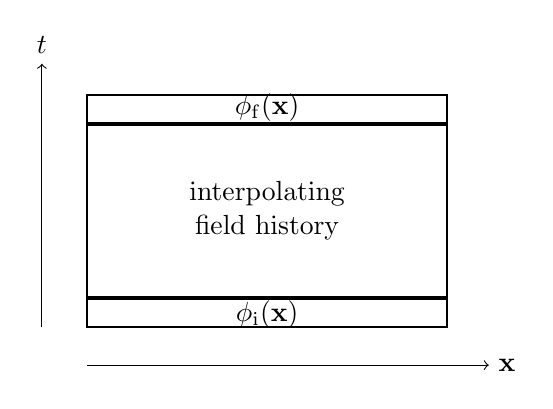
\begin{tikzpicture}[scale=0.88]
\draw[->] (-0.65,0) -- (-0.65,3.8) node[above] {$t$};
\draw[->] (0,-0.55) -- (5.8,-0.55) node[right] {$\mathbf{x}$};
\draw[thick] (0,0) rectangle (5.2,3.35);
\draw[very thick] (0,0.42) -- (5.2,0.42);
\draw[very thick] (0,2.93) -- (5.2,2.93);
\node at (2.6,0.18) {$\phi_{\mathrm{i}}(\mathbf{x})$};
\node at (2.6,3.17) {$\phi_{\mathrm{f}}(\mathbf{x})$};
\node[align=center] at (2.6,1.68) {interpolating\\field history};
\end{tikzpicture}
\caption{Anfangs- und Endkonfiguration des Feldes begrenzen ein Raumzeitgebiet.}
\end{figure}

\begin{classroomqa}
\lecturetimestamp{00:07:34}
\audiencequestion{Kann ein Feld wieder denselben Wert annehmen?}
\lecturerresponse{Ja. Es gibt kein Hindernis dafür, dass ein Feld wieder einen früheren Wert annimmt, genauso wenig wie dafür, dass eine Teilchenkoordinate wieder eine frühere Position erreicht.}
\end{classroomqa}

\begin{classroomqa}
\lecturetimestamp{00:07:46}
\audiencequestion{Warum spricht man von Raumzeitereignissen oder einer Bahn, wenn die Randdaten Feldwerte sind?}
\lecturerresponse{An die Stelle der Teilchenbahn tritt eine Feldgeschichte. Jeder Endpunkt im Feldraum ist das vollständige Feld auf einer gewählten Zeitscheibe, und eine Geschichte gibt das Feld an jedem Punkt des Raumzeitgebiets zwischen den beiden Scheiben an.}
\end{classroomqa}

Die Forderung nach stationärer Wirkung für das interpolierende Feld führt auf partielle Differentialgleichungen. Je nach Feldern und Lagrange-Funktion gehören dazu etwa die Maxwell-Gleichungen und, bei einer Gravitationswirkung, die Einstein-Gleichungen. Die ausführliche Variationsrechnung benötigen wir hier nicht; entscheidend ist die folgende Abfolge:
\begin{equation}
\mathcal{L}
\longrightarrow
S[\phi]
\longrightarrow
\text{classical field equations}.
\end{equation}

\section{Feynmans Summe über Teilchenbahnen}

In der Quantenmechanik wird die Frage, welche Bahn eintritt, durch eine Frage nach Amplituden ersetzt. Stellen wir uns vor, bei \((x,t)\) ein Teilchen einzuspeisen, eine Weile die Augen zu schließen und dann bei \((x',t')\) einen Detektor einzuschalten. Die Amplitude
\begin{equation}
\mathcal{A}(x,t;x',t')
\end{equation}
ist eine komplexe Zahl. Ihr Betragsquadrat ist die Wahrscheinlichkeit:
\begin{equation}
\begin{aligned}
P(x,t;x',t')
&=\left|\mathcal{A}(x,t;x',t')\right|^2\\
&=\mathcal{A}(x,t;x',t')
\mathcal{A}(x,t;x',t')^*.
\end{aligned}
\end{equation}

Nach Feynmans Vorschrift wird jeder möglichen Bahn eine Wirkung zugeordnet und ihr die Phase
\begin{equation}
\exp\!\left(-\frac{i}{\hbar}S[x]\right)
=
\exp\!\left[-\frac{i}{\hbar}\int \mathcal{L}(x,\dot{x})\,dt\right].
\end{equation}

\begin{figure}[htbp]
\centering
\includegraphics[width=0.70\textwidth]{lecture_10_figure_04.png}
\caption{Komplexe Phase zu einer Teilchenbahn.}
\lectureframe{00:11:52}
\end{figure}

Der Faktor \(\hbar\) ist nötig, damit der Exponent dimensionslos ist.\footnote{Auf der Tafel steht bei 00:11:52 plausibel \(e^{-i\int\mathcal{L}\,dt}\); der Faktor \(\hbar\) wird mündlich bei 00:12:02 ergänzt.} Die Übergangsamplitude ist die Summe dieser Phasen über alle möglichen Bahnen, die die Endpunkte verbinden:
\begin{equation}
\mathcal{A}(x,t;x',t')
=
\sum_{\substack{\text{paths }x(\tau)\\(x,t)\rightarrow(x',t')}}
\exp\!\left(-\frac{i}{\hbar}S[x]\right).
\end{equation}
Hier bedeutet ``mögliche Bahn'' nicht eine Lösung der Newtonschen Gleichungen. Gemeint ist jede Bahn, die in die Summe eingeht. In der nichtrelativistischen Quantenmechanik verlaufen die Bahnen in Vorwärtsrichtung der Zeit und bilden keine Schleifen rückwärts in der Zeit. Das Plancksche Wirkungsquantum hat die Dimension einer Wirkung, daher ist \(S/\hbar\) dimensionslos.

Die Exponentialfunktion ist naheliegend, weil sich die Amplituden aufeinanderfolgender kleiner Schritte multiplizieren. Wird eine Bahn in aufeinanderfolgende Abschnitte unterteilt, addieren sich die Wirkungen,
\begin{equation}
S=S_1+S_2+\cdots,
\end{equation}
während sich die Phasen multiplizieren:
\begin{equation}
e^{-iS/\hbar}
=e^{-iS_1/\hbar}e^{-iS_2/\hbar}\cdots.
\end{equation}
Der Faktor \(i\) ist keine bloße Rechenkonvention, sondern gehört zur quantenmechanischen Vorschrift.

\begin{classroomqa}
\lecturetimestamp{00:13:27}
\audiencequestion{Hängt die Exponentialfunktion damit zusammen, dass man die Amplituden aufeinanderfolgender kleiner Schritte multipliziert?}
\lecturerresponse{Ja. Die Amplituden aufeinanderfolgender Schritte multiplizieren sich, während sich die zugehörigen Wirkungsanteile addieren.}
\end{classroomqa}

\begin{classroomqa}
\lecturetimestamp{00:13:49}
\audiencequestion{Ist die Summe über die Bahnen selbst die Wahrscheinlichkeit?}
\lecturerresponse{Nein. Die Summe über die Bahnen ist im Allgemeinen eine komplexe Wahrscheinlichkeitsamplitude. Multipliziert man sie mit ihrer komplex konjugierten Zahl, erhält man die Wahrscheinlichkeit.}
\end{classroomqa}

\section{Die Summe über Feldgeschichten}

Dieselbe Formulierung lässt sich auf die Quantenfeldtheorie übertragen, auch wenn die folgende Konstruktion bewusst nicht streng mathematisch sein wird. Beginnen wir mit einer anfänglichen Feldkonfiguration \(\phi(\mathbf{x})\) und einer unabhängig davon festgelegten Endkonfiguration \(\phi'(\mathbf{x})\). Es handelt sich um vollständige Funktionen des Raums, nicht um Werte an zwei isolierten Punkten.

Man kann sich einen idealisierten Apparat vorstellen, der das Feld an jedem Raumpunkt präpariert, das System sich entwickeln lässt und später das Feld überall misst. Ein solcher Apparat ist unrealistisch, doch er formuliert die konzeptionelle Frage klar: Wie groß ist die Amplitude für den Übergang von der vollständigen anfänglichen Feldkonfiguration zur vollständigen Endkonfiguration?

Jede denkbare interpolierende Feldgeschichte trägt bei. Für jede Geschichte berechnet man
\begin{equation}
S[\phi]=\int d^4x\,\mathcal{L}(\phi,\partial_\mu\phi)
\end{equation}
und versieht sie mit der entsprechenden Phase. Schematisch gilt:
\begin{equation}
\mathcal{A}\!\left[\phi(\mathbf{x})\rightarrow\phi'(\mathbf{x})\right]
=
\sum_{\substack{\text{field histories}\\
\phi_{\mathrm{i}}=\phi,\;\phi_{\mathrm{f}}=\phi'}}
\exp\!\left(-\frac{i}{\hbar}S[\phi]\right).
\end{equation}
Eine Geschichte muss die klassischen Feldgleichungen nicht erfüllen. Sie ist lediglich eine vollständige Zuordnung von Feldwerten im gesamten dazwischenliegenden Raumzeitgebiet.

\begin{classroomqa}
\lecturetimestamp{00:17:39}
\audiencequestion{Es gibt unendlich viele Geschichten, und jede Phase hat den Betrag eins. Wie kann ihre Summe konvergieren? Werden die Geschichten minimiert?}
\lecturerresponse{Die Geschichten werden summiert, nicht minimiert. Die Summanden sind Phasen, die auf dem Einheitskreis verteilt sind und sich daher gegenseitig aufheben können. Das unterscheidet sich von der Addition unendlich vieler positiver Terme, die von null weg beschränkt sind. Oszillierende Integrale können konvergieren; die Fourier-Darstellung der Deltafunktion ist ein bekanntes Beispiel. Wären die Phasen gleichmäßig auf dem Kreis verteilt, wäre ihre Vektorsumme null. Die meisten Geschichten heben sich weitgehend gegenseitig auf. Geschichten in der Nähe einer Bahn mit stationärer Wirkung löschen sich am wenigsten aus, weil sich die Phase dort am langsamsten ändert. So ergibt sich der klassische Grenzfall.}
\end{classroomqa}

\editorialnote{Ein Pfadintegral in reeller Zeit erfordert üblicherweise eine Vorschrift zur Sicherung der Konvergenz. Die Betrachtung auf dem Einheitskreis veranschaulicht hier das Argument der oszillatorischen Auslöschung, ist aber kein allgemeiner Konvergenzbeweis.}

Die Auslöschung lässt sich als Vektorsumme in der komplexen Ebene veranschaulichen.\footnote{Die Konstruktion mit dem Einheitskreis wird anhand der Tafelbesprechung bei 00:18:32--00:20:21 rekonstruiert.}
\begin{figure}[htbp]
\centering
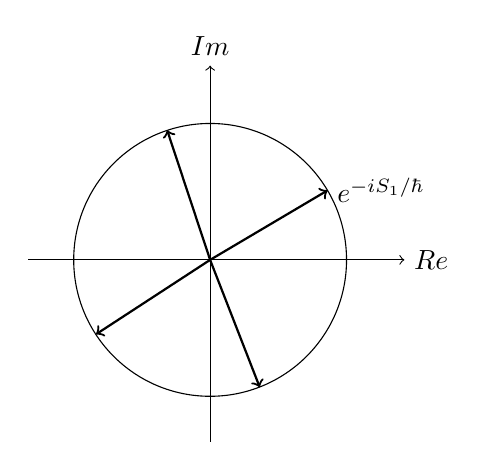
\begin{tikzpicture}[scale=1.05]
\draw[->] (-2.2,0) -- (2.35,0) node[right] {$\operatorname{Re}$};
\draw[->] (0,-2.2) -- (0,2.35) node[above] {$\operatorname{Im}$};
\draw (0,0) circle (1.65);
\draw[thick,->] (0,0) -- (1.42,0.84);
\draw[thick,->] (0,0) -- (-1.38,-0.90);
\draw[thick,->] (0,0) -- (-0.52,1.57);
\draw[thick,->] (0,0) -- (0.60,-1.54);
\node[right] at (1.42,0.84) {$e^{-iS_1/\hbar}$};
\end{tikzpicture}
\caption{Phasen mit Einheitsbetrag können sich bei unterschiedlichen Richtungen gegenseitig aufheben.}
\end{figure}

Tatsächlich gilt:
\begin{equation}
e^{-iS/\hbar}
=
\cos\!\left(\frac{S}{\hbar}\right)
-i\sin\!\left(\frac{S}{\hbar}\right).
\end{equation}
Jeder Beitrag ist ein Einheitsvektor. Beiträge in verschiedene Richtungen können sich sowohl addieren als auch gegenseitig aufheben. In der Nähe eines stationären Punktes von \(S\) haben benachbarte Geschichten nahezu dieselbe Phase, sodass sich ihre Beiträge wirksamer verstärken. Abseits stationärer Wirkung ändert sich die Phase rasch, und destruktive Interferenz überwiegt.

Diese Pfadintegralstruktur liegt im Wesentlichen der gesamten modernen Quantenfeldtheorie zugrunde. Der nächste praktische Schritt wird angegeben, nicht hergeleitet. Dieser stark vereinfachte Zugang zur Rechnung macht jedoch sichtbar, wie sich dasselbe Objekt in zwei verschiedenen Sprachen verwenden lässt.

Einen Prozess zu berechnen heißt, eine Übergangswahrscheinlichkeit vom Anfangs- zum Endzustand zu berechnen. Eine Beschreibung legt eine anfängliche und eine abschließende Feldkonfiguration fest. Die andere beschreibt ein- und auslaufende Teilchen, also die Quanten eines oder mehrerer Felder. Diese Fragen sehen verschieden aus, werden aber beide mit demselben quantenfeldtheoretischen Pfadintegral berechnet.

\section{Eine diskrete Raumzeitdarstellung}

Um der Summe über Feldgeschichten eine konkrete Bedeutung zu geben, unterteilen wir die Raumzeit in kleine Zellen und ordnen jeder Zelle einen Feldwert zu. Dem Kontinuum nähern wir uns, indem wir die Zellgröße verkleinern; vorerst bleiben die Zellen jedoch endlich. Dadurch wird die formale Summe über Funktionen zu einer Summe über Zahlenzuordnungen auf den Gitterzellen.

Eine frühere heuristische Betrachtung verwendet für jede Zelle ein Produkt von Faktoren ähnlich \(1+\mathcal{L}_i\) und identifiziert dann Terme, die Teilchenpropagation und Kollisionen beschreiben. Da diese Konstruktion zentral ist, wiederholen wir sie, müssen den Faktor aber korrigieren. Die kleine Größe ist nicht die Lagrange-Funktion selbst, sondern die in einer Zelle enthaltene Wirkung.

Hat eine Zelle das Raumzeitvolumen
\begin{equation}
a^4=\Delta t\,\Delta x\,\Delta y\,\Delta z,
\end{equation}
so ist ihre Wirkung
\begin{equation}
A_i=\mathcal{L}_i a^4.
\end{equation}
Da die Zelle klein ist, ist auch \(A_i\) klein. Lassen wir \(\hbar\) vorübergehend weg, lautet der korrigierte elementare Faktor
\begin{equation}
1-iA_i,
\end{equation}
und nicht \(1+\mathcal{L}_i\).

Für ein beliebig kleines \(\epsilon\) gilt
\begin{equation}
1+\epsilon\simeq e^\epsilon,
\end{equation}
weil
\begin{equation}
e^\epsilon
=1+\epsilon+\frac{\epsilon^2}{2!}
+\frac{\epsilon^3}{3!}+\cdots.
\end{equation}
Somit nähert \(1-iA_i\) in diesen vorübergehend gewählten Einheiten für eine hinreichend kleine Zelle \(e^{-iA_i}\) an. Es ist klarer, von Anfang an den exakten Exponentialfaktor zu verwenden.

\begin{classroomqa}
\lecturetimestamp{00:27:57}
\audiencequestion{Benötigt die Exponentialfunktion einen Faktor \(\hbar\)?}
\lecturerresponse{Ja. Der dimensionslose Zellfaktor lautet in erster Ordnung \(1-iA_i/\hbar\), und der exakte Exponentialfaktor ist \(\exp(-iA_i/\hbar)\). Später kann man Einheiten wählen, in denen \(\hbar=1\) gilt.}
\end{classroomqa}

Mit wieder eingesetztem \(\hbar\) lauten der korrigierte Zwischenfaktor und seine Exponentialform:
\begin{equation}
1-\frac{i}{\hbar}A_i
\simeq
\exp\!\left(-\frac{i}{\hbar}A_i\right).
\end{equation}

Für eine feste Geschichte ersetzt man das Raumzeitintegral durch eine Summe der Zellwirkungen:
\begin{equation}
S[\phi]
=\int d^4x\,\mathcal{L}
\;\longrightarrow\;
\sum_i A_i.
\end{equation}
Die Phase dieser Geschichte lautet dann
\begin{equation}
\exp\!\left(-\frac{i}{\hbar}\sum_i A_i\right).
\end{equation}
Eine Exponentialfunktion einer Summe ist ein Produkt von Exponentialfunktionen:
\begin{equation}
\exp\!\left(-\frac{i}{\hbar}\sum_i A_i\right)
=
\prod_i\exp\!\left(-\frac{i}{\hbar}A_i\right).
\end{equation}
Die Reihenfolge der Operationen ist wichtig. Zuerst wählt man eine vollständige Geschichte aus und multipliziert ihre Zellgewichte. Erst danach summiert man über die verschiedenen Geschichten.

Auch die Randdaten werden auf dem Gitter explizit.\footnote{Das Schachbrettmuster mit festgelegter erster und letzter Reihe wird anhand der Abbildungen bei ungefähr 00:23:54 und 00:30:49 rekonstruiert.}
\begin{figure}[htbp]
\centering
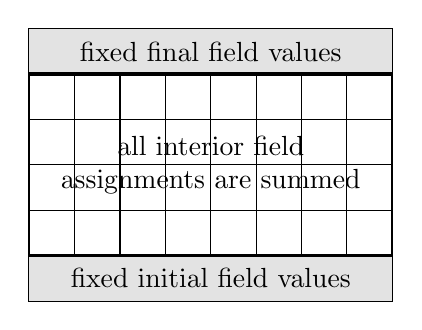
\begin{tikzpicture}[scale=0.72]
\draw[step=0.8,thin] (0,0) grid (6.4,4.8);
\draw[thick] (0,0) rectangle (6.4,4.8);
\fill[gray!22] (0,0) rectangle (6.4,0.8);
\fill[gray!22] (0,4.0) rectangle (6.4,4.8);
\draw[very thick] (0,0.8) -- (6.4,0.8);
\draw[very thick] (0,4.0) -- (6.4,4.0);
\node at (3.2,0.4) {fixed initial field values};
\node at (3.2,4.4) {fixed final field values};
\node[align=center] at (3.2,2.4) {all interior field\\assignments are summed};
\end{tikzpicture}
\caption{Diskrete Feldgeschichten mit festen anfänglichen und abschließenden Gitterreihen.}
\end{figure}

Die erste Reihe legt die anfängliche Feldkonfiguration fest, die letzte die abschließende. Jeder inneren Zelle ist jeder Feldwert erlaubt, der in der Diskretisierung enthalten ist. Die Übergangsamplitude hat daher schematisch die Form
\begin{equation}
\mathcal{A}\!\left[\phi_{\mathrm{i}}\rightarrow\phi_{\mathrm{f}}\right]
=
\sum_{\{\phi\}_{\mathrm{interior}}}
\prod_i\exp\!\left(-\frac{i}{\hbar}A_i[\phi]\right),
\end{equation}
wobei die erste und letzte Reihe festgehalten werden. Gleichwertig berechnet man für jede Zuordnung im Inneren die Exponentialfunktion der Gesamtwirkung und addiert diesen Beitrag zu den Beiträgen aller anderen Zuordnungen.

\section{Von Feldkonfigurationen zu Teilchenkonfigurationen}

Dieselbe Übergangsamplitude lässt sich mit Feldern oder mit Teilchen beschreiben. Statt das Feld auf der ersten und letzten Zeitscheibe festzulegen, kann man einlaufende und auslaufende Ansammlungen von Feldquanten vorgeben und nach der Amplitude fragen, die sie verbindet. Berechnet wird dasselbe Objekt. Lediglich die Beschreibung der Randbedingungen hat sich geändert.

Quantenfelder enthalten Erzeugungs- und Vernichtungsoperatoren. Produkte von Feldern wirken daher auf Teilchenzustände, indem sie Quanten erzeugen, vernichten oder ihren Ort ändern. Diese Operatorinterpretation führt von dem Gitterpfadintegral zu den Teilchenregeln.

\begin{classroomqa}
\lecturetimestamp{00:34:11}
\audiencequestion{Sind Feldquanten notwendigerweise als Teilchen identifizierbar?}
\lecturerresponse{Nicht immer im herkömmlichen Sinn separat beobachtbarer Teilchen. Quarks sind beispielsweise Quanten von Quarkfeldern, doch aufgrund des Confinements kann ein isoliertes Quark nicht entkommen und für sich allein nachgewiesen werden. Allgemeiner muss es keine Eins-zu-eins-Zuordnung zwischen den in einer Theorie bezeichneten Feldern und den Teilchenspezies geben, die als gewöhnliche beobachtbare Zustände auftreten. Manche Feldtheorien lassen eine solche einfache Zuordnung nicht zu. Verwendet man ``Teilchen'' in einem weiten Sinn für ein unteilbares Quant, das Energie und andere Quantenzahlen trägt, kann der Unterschied teilweise zu einer Frage der Terminologie werden.}
\end{classroomqa}

\editorialnote{Die Aussage der Quelle zur schwachen Kopplung bei 00:35:45--00:36:08 ist grammatisch mehrdeutig und wird hier nicht aufgelöst. Sicher ist die Aussage, dass Feldbezeichnungen und herkömmliche beobachtbare Teilchenspezies nicht notwendigerweise einander eindeutig zugeordnet sind.}

Die Gittersumme erstreckt sich weiterhin über Feldwerte. Sie ist nicht auf Konfigurationen beschränkt, die glatten klassischen Lösungen ähneln.

\begin{classroomqa}
\lecturetimestamp{00:36:44}
\audiencequestion{Müssen die Feldgeschichten stetig oder zumindest näherungsweise stetig sein?}
\lecturerresponse{Nein. Auf einem diskreten Gitter tragen benachbarte Zellen einfach Feldwerte, und jede Zuordnung geht in die Summe ein. Es gibt keine Beschränkung auf näherungsweise stetige Geschichten. Quantenfelder fluktuieren stark; typische Geschichten sind keine glatten klassischen Felder.}
\end{classroomqa}

Unabhängig zugewiesen werden die Felder an den Gitterstellen oder -zellen. Ihre Ableitungen ergeben sich aus Differenzen benachbarter Werte.

\begin{classroomqa}
\lecturetimestamp{00:37:56}
\audiencequestion{Werden den Feldern und ihren Ableitungen unabhängige Werte zugewiesen?}
\lecturerresponse{Nein. Die Feldwerte werden an den Gitterstellen festgelegt. Eine Ableitung wird anschließend aus der Differenz benachbarter Feldwerte rekonstruiert. Es gibt verschiedene Möglichkeiten, endliche Differenzen zu definieren, aber die Ableitungen sind keine zusätzlichen unabhängigen Variablen.}
\end{classroomqa}

Für den Gitterabstand \(a\) kann man also schematisch schreiben:
\begin{equation}
\partial_\mu\phi(x)
\longrightarrow
\frac{\phi(x+a\hat\mu)-\phi(x)}{a}.
\end{equation}
Auch die Achse der Feldwerte lässt sich in kleine Intervalle unterteilen, sodass an jeder Gitterstelle eine abzählbare Menge möglicher Werte verbleibt.

\begin{classroomqa}
\lecturetimestamp{00:38:53}
\audiencequestion{Was ändert sich, wenn es mehr als ein Feld gibt?}
\lecturerresponse{An jeder Gitterstelle wird jedem Feld ein Wert zugeordnet, und die Summe erstreckt sich über alle solchen Zuordnungen.}
\end{classroomqa}

Ein komplexwertiges Feld ist nicht mit einer analytischen Funktion einer komplexen Variablen zu verwechseln. Analytizität ist eine außergewöhnlich starke Glattheitsbedingung. Die Geschichten in einem Feldpfadintegral müssen sie nicht erfüllen und sind im Allgemeinen nicht einmal näherungsweise glatt.

\begin{classroomqa}
\lecturetimestamp{00:39:07}
\audiencequestion{Müssen die Werte komplexwertiger Felder die Glattheitsbedingungen erfüllen, denen analytische Funktionen genügen?}
\lecturerresponse{Nein. Komplexwertig bedeutet nicht analytisch. Die Funktionentheorie behandelt eine äußerst glatte und stark eingeschränkte Klasse von Funktionen. Die hier summierten Feldgeschichten müssen keine analytischen Funktionen des Ortes sein; typische Geschichten sind sehr irregulär und können im Kontinuumslimes als stark unstetig angesehen werden.}
\end{classroomqa}

Die daraus entstehende Rechnung wirkt gewaltig. Selbst nachdem Raumzeit und Feldwerte diskretisiert wurden, kann es eine enorme Zahl von Zuordnungen geben, die abgetastet werden müssen.

\begin{classroomqa}
\lecturetimestamp{00:40:04}
\audiencequestion{Woher weiß ein Computer, wie viele Gitterzuordnungen abzutasten sind oder wann die Rechnung konvergiert ist?}
\lecturerresponse{Diese Frage gehört zur Gittereichtheorie oder allgemeiner zur Gitterquantenfeldtheorie. Inzwischen ist sie ein leistungsfähiges Rechengebiet. Ich war ganz am Anfang an der Aufstellung der Regeln für die Gittereichtheorie beteiligt, nicht an der späteren Computertechnik. Die Regeln aufzustellen dauerte etwa drei Wochen; die Entwicklung der Technik zur Berechnung solcher Größen dauerte etwa dreißig Jahre. Ein großer Teil des praktischen Wissens stammt aus der statistischen Mechanik, wo Zustandssummen ebenfalls durch Summieren über Gitterkonfigurationen berechnet werden---zum Beispiel darüber, ob eine Gitterstelle in einem Kristall besetzt ist. Ob genügend Konfigurationen abgetastet wurden, ist eine technische Frage. Die Fachleute wissen---oder glauben zu wissen---, wann die Rechnung unter Kontrolle ist, und die Ergebnisse stimmen mit dem Experiment überein.}
\end{classroomqa}

Die konzeptionellen Regeln für die Gittereichtheorie waren schnell aufgestellt; die dafür nötige Rechentechnik erforderte wesentlich mehr Zeit. Das Schachbrett ist nicht bloß ein Vergleich. Es ist auch der Ausgangspunkt einer praktischen Rechenmethode.

\section{Quadratische Terme und Teilchenpropagation}

Kehren wir nun zur Operatorinterpretation der Felder zurück. Für zwei benachbarte Gitterstellen \(x\) und \(x'\) kann das Produkt
\begin{equation}
\phi(x)\phi(x')
\end{equation}
in einem geeigneten Einteilchen-Matrixelement die Vernichtung eines Teilchens an der einen Stelle und seine Erzeugung an der anderen bewirken. In diesem Teilchensektor lässt es sich daher als Sprung über eine Gitterkante auffassen. Dies ist eine mögliche Interpretation des Operatorprodukts, aber nicht seine einzige.

Die für solche Verbindungen verantwortlichen Terme sind die Ableitungsterme. Genau genommen gehören sie nicht zu einer einzelnen Zelle, sondern zu einem Paar benachbarter Zellen. Eine zeitliche Ableitung wird beispielsweise zu
\begin{equation}
\partial_t\phi(t,\mathbf{x})
\longrightarrow
\frac{\phi(t+a,\mathbf{x})-\phi(t,\mathbf{x})}{a},
\end{equation}
Eine räumliche Ableitung behandelt man entsprechend entlang einer räumlichen Gitterkante.

\begin{classroomqa}
\lecturetimestamp{00:44:39}
\audiencequestion{Enthalten die hier behandelten Lagrange-Funktionen zweite Ableitungen?}
\lecturerresponse{Die hier betrachteten Standardtheorien sind mit ersten Ableitungen formuliert. Ihre Gitterversionen verwenden daher erste Differenzen zwischen benachbarten Gitterstellen.}
\end{classroomqa}

Das Quadrieren einer ersten Differenz ergibt sowohl Terme an derselben Gitterstelle als auch einen gemischten Term für benachbarte Stellen:
\begin{align}
\frac{1}{2}\bigl[\phi(x)-\phi(x')\bigr]^2
&=
\frac{1}{2}\phi(x)^2
+\frac{1}{2}\phi(x')^2
-\phi(x)\phi(x').
\end{align}
Der gemischte Term kann eine Bewegung von einer Gitterstelle zur anderen ermöglichen. Die beiden Quadrate sind Terme an jeweils derselben Gitterstelle. Die quadratischen Ableitungsterme sind die kinetischen Terme; zunächst verwenden wir ihre gemischten Terme für benachbarte Stellen, um die Propagation aufzubauen.

Um die Kombinatorik herauszustellen, fassen wir die Produkte benachbarter Feldwerte zusammen zu
\begin{equation}
K=\sum_{\langle x,x'\rangle}\phi(x)\phi(x').
\end{equation}
Der zugehörige Faktor im Pfadintegralgewicht wird schematisch geschrieben als
\begin{equation}
e^{-iK}.
\end{equation}
\editorialnote{In diesem schematischen Gitterfaktor sind Potenzen des Gitterabstands, \(\hbar\), Vorzeichen aus der Metrik, Normierungskonstanten und Koeffizienten der Verbindungen unterdrückt.}
Die Entwicklung lautet
\begin{equation}
e^{-iK}
=1-iK-\frac{1}{2!}K^2+\frac{i}{3!}K^3+\cdots,
\end{equation}
oder, mit ausgeschriebenen Summen über Nachbarstellen,
\begin{align}
e^{-iK}
={}&1
-i\sum_{\langle x,x'\rangle}\phi(x)\phi(x')
\nonumber\\
&-\frac{1}{2!}
\sum_{\langle x,x'\rangle}
\sum_{\langle y,y'\rangle}
\phi(x)\phi(x')\phi(y)\phi(y')
+\cdots .
\end{align}
Jeder Faktor wählt unabhängig ein Paar benachbarter Stellen aus.

Für die Teilchendiagramme gilt eine Regel gegen offene Enden. Ein freier Endpunkt ist nur dort zulässig, wo die Randbedingung ausdrücklich ein Teilchen auf der anfänglichen Scheibe einfügt oder es auf der abschließenden Scheibe entfernt. Eine isolierte Verbindung im Inneren hat nicht verbundene Enden und stellt keinen vollständigen Beitrag zum vorgegebenen Übergang dar. Die inneren Enden der Verbindungen müssen zusammengefügt werden.

Betrachten wir zunächst ein Gitter mit nur zwei Zeitschichten. Fügt der Anfangszustand bei \(x\) ein Teilchen ein und entfernt der Endzustand es am benachbarten Punkt \(x'\), kann der Term erster Ordnung die beiden Randoperationen verbinden:
\begin{equation}
x\longrightarrow x',
\qquad
\mathcal{A}_{\text{one link}}\sim -i.
\end{equation}
Der Koeffizient \(-i\) ist lediglich der Koeffizient in dieser schematischen Entwicklung; die unterdrückten Gitter- und Normierungsfaktoren sind weiterhin mitgemeint.

\begin{classroomqa}
\lecturetimestamp{00:52:16}
\audiencequestion{Trägt der Term erster Ordnung mit einer Gitterkante nur dann bei, wenn die betreffenden Anfangs- und Endstellen benachbart sind?}
\lecturerresponse{Ja. Dieser Term wählt ein Paar benachbarter Stellen aus und kann diese Randstellen daher nur verbinden, wenn sie Nachbarn sind. Propagation über größere Abstände ergibt sich aus Produkten höherer Ordnung.}
\end{classroomqa}

In zweiter Ordnung wird jeder der beiden Faktoren unabhängig über benachbarte Paare summiert:
\begin{equation}
K^2
=
\sum_{\langle x,x'\rangle}
\sum_{\langle y,y'\rangle}
\phi(x)\phi(x')\phi(y)\phi(y').
\end{equation}

\begin{classroomqa}
\lecturetimestamp{00:52:40}
\audiencequestion{Muss das zweite Paar benachbarter Stellen an das vom ersten Faktor gewählte Paar angrenzen?}
\lecturerresponse{Nein. Jeder Faktor wählt unabhängig ein Paar benachbarter Stellen aus. Die beiden Paare können eine Stelle gemeinsam haben, vollständig getrennt sein oder sogar dasselbe Paar sein. Die Summe umfasst alle Möglichkeiten.}
\end{classroomqa}

Für ein Teilchen, das sich über drei Zeitschichten ausbreitet, ist in zweiter Ordnung die Auswahl mit einer gemeinsamen Zwischenstelle relevant:
\begin{equation}
\bigl[\phi(x_0)\phi(x_1)\bigr]
\bigl[\phi(x_1)\phi(x_2)\bigr],
\qquad
x_0\longrightarrow x_1\longrightarrow x_2.
\end{equation}
Das Ende der ersten Verbindung wird mit dem Anfang der zweiten zusammengefügt. Nur der Anfangspunkt bei \(x_0\) und der Endpunkt bei \(x_2\) bleiben frei; daher trägt dieser Term zum gesuchten Einteilchenübergang bei. In der schematischen Exponentialfunktion ist sein Koeffizient
\begin{equation}
-\frac{1}{2!}.
\end{equation}

Stattdessen können die ausgewählten Verbindungen auch getrennte Sprünge bilden.\footnote{Die Verbindungsdiagramme werden anhand der Abfolge bei 00:49:18--00:55:12 rekonstruiert.}
\begin{figure}[htbp]
\centering
\resizebox{\linewidth}{!}{%
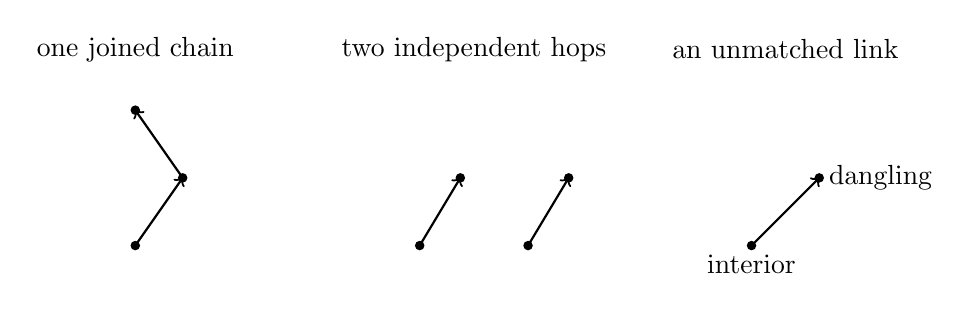
\begin{tikzpicture}[scale=0.86]
\node at (0,2.9) {one joined chain};
\fill (0,0) circle (2pt);
\fill (0.7,1.0) circle (2pt);
\fill (0,2.0) circle (2pt);
\draw[thick,->] (0,0) -- (0.7,1.0);
\draw[thick,->] (0.7,1.0) -- (0,2.0);

\begin{scope}[xshift=4.2cm]
\node at (0.8,2.9) {two independent hops};
\fill (0,0) circle (2pt);
\fill (0.6,1.0) circle (2pt);
\fill (1.6,0) circle (2pt);
\fill (2.2,1.0) circle (2pt);
\draw[thick,->] (0,0) -- (0.6,1.0);
\draw[thick,->] (1.6,0) -- (2.2,1.0);
\end{scope}

\begin{scope}[xshift=9.1cm]
\node at (0.5,2.9) {an unmatched link};
\fill (0,0) circle (2pt);
\fill (1.0,1.0) circle (2pt);
\draw[thick,->] (0,0) -- (1.0,1.0);
\node[below] at (0,0) {interior};
\node[right] at (1.0,1.0) {dangling};
\end{scope}
\end{tikzpicture}%
}
\caption{Zusammengefügte und unabhängige Auswahlen benachbarter Verbindungen sowie Auswahlen mit offenen Enden.}
\end{figure}

Schon in dieser Ordnung kann es mehr als einen Weg geben. Bei einer Verschiebung um je einen zeitlichen und räumlichen Gitterschritt führen die beiden Reihenfolgen
\begin{align}
x
&\longrightarrow x+\hat t
\longrightarrow x+\hat t+\hat s,\\
x
&\longrightarrow x+\hat s
\longrightarrow x+\hat s+\hat t
\end{align}
zum selben Endpunkt.

\begin{classroomqa}
\lecturetimestamp{00:55:53}
\audiencequestion{Gibt es noch einen anderen Weg mit zwei Schritten zum selben diagonalen Endpunkt?}
\lecturerresponse{Ja. Man kann zuerst den zeitlichen und dann den räumlichen Schritt ausführen oder die Schritte in umgekehrter Reihenfolge gehen. Beide Wege tragen zur selben Übergangsamplitude bei.}
\end{classroomqa}

Es gibt keinen Grund, bei zwei Verbindungen aufzuhören. Der Term dritter Ordnung liefert Ketten aus drei benachbarten Verbindungen. Ein Weg kann direkt voranschreiten, einen Umweg nehmen oder sich zunächst vom Endpunkt entfernen und wieder zurückkehren. Noch höhere Ordnungen umfassen längere Umwege und wiederholtes Zurücklaufen. Die Entwicklung bis zu beliebiger Ordnung liefert daher einen Beitrag für jeden Weg, der aus lokalen Verbindungen zusammengesetzt ist. Die Amplitude von Punkt zu Punkt ist die Summe all dieser Beiträge; ihre Koeffizienten enthalten die entsprechenden Potenzen von \(i\) und Fakultäten:
\begin{equation}
\begin{gathered}
\mathcal{A}(x_{\mathrm{in}}\to x_{\mathrm{out}})
=
\sum_{\text{joined lattice routes }r}c_r,
\\
c_r\ \hbox{read from the exponential expansion}.
\end{gathered}
\end{equation}
Die Koeffizienten sind im Allgemeinen komplex, daher ist auch die resultierende Amplitude komplex.

Bei relativistischer Propagation kommt noch eine Möglichkeit hinzu. Ein Weg kann sowohl in zeitlicher Vorwärts- als auch in Rückwärtsrichtung verlaufen und dieselbe Verbindung wiederholt durchlaufen.

\begin{classroomqa}
\lecturetimestamp{00:58:47}
\audiencequestion{Kann ein Weg immer wieder durch dieselben beiden Zellen führen?}
\lecturerresponse{Ja. Wiederholte Durchläufe sind enthalten, und in der relativistischen Entwicklung kann der Weg auch rückwärts in der Zeit verlaufen.}
\end{classroomqa}

Ein zeitlich rückwärts gerichteter Abschnitt lässt sich grafisch auf zwei gleichwertige Arten lesen. Man kann ihn als Teilchenlinie auffassen, die rückwärts in der Zeit verläuft. Oder man betrachtet die Zeit nur vorwärts: Ein Teilchen--Antiteilchen-Paar wird erzeugt, das Teilchen bewegt sich weiter vorwärts, und das Antiteilchen trifft später auf das ursprüngliche Teilchen und vernichtet es. Dieselbe zusammenhängende Linie kodiert beide Beschreibungen.\footnote{Die beiden Lesarten folgen dem Diagramm und der Erläuterung bei 00:59:00--00:59:51.}

\begin{figure}[htbp]
\centering
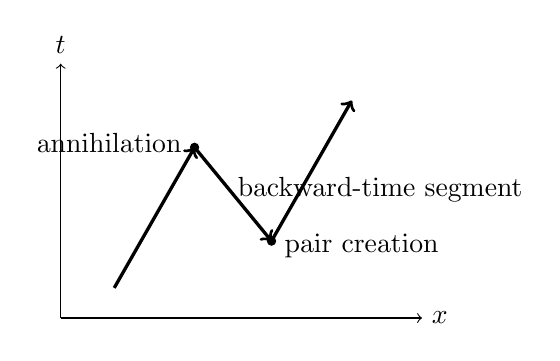
\begin{tikzpicture}[scale=0.85]
\draw[->] (0,0) -- (0,3.8) node[above] {$t$};
\draw[->] (0,0) -- (5.4,0) node[right] {$x$};
\draw[very thick,->] (0.8,0.45) -- (2.0,2.55);
\draw[very thick,->] (2.0,2.55) -- (3.15,1.15);
\draw[very thick,->] (3.15,1.15) -- (4.35,3.25);
\fill (2.0,2.55) circle (2pt);
\fill (3.15,1.15) circle (2pt);
\node[left] at (1.95,2.62) {annihilation};
\node[right] at (3.20,1.08) {pair creation};
\node[right] at (2.50,1.92) {backward-time segment};
\end{tikzpicture}
\caption{Ein zeitlich rückwärts gerichteter Abschnitt, vorwärts gelesen als Paarerzeugung und Vernichtung.}
\end{figure}

Die bei hohen Ordnungen auftretenden Fakultäten kontrollieren die exponentielle Potenzreihe. Das ist jedoch nicht dasselbe, wie die gesamte Summe über die Feldkonfigurationen zu kontrollieren.

\begin{classroomqa}
\lecturetimestamp{01:00:00}
\audiencequestion{Garantieren die Faktoren \(1/n!\) Konvergenz?}
\lecturerresponse{Sie garantieren die Konvergenz der Exponentialreihe für ein festes Argument. Für sich allein garantieren sie nicht die Konvergenz der separaten Summe über alle Feldkonfigurationen. Das sind verschiedene Fragen. Auf einem endlichen Gitter mit einer endlichen diskretisierten Menge von Feldwerten ist die Zahl der Konfigurationen endlich; die Kontinuums- und unendlichen Volumengrenzwerte erfordern jedoch weitere Kontrolle.}
\end{classroomqa}

\section{Ein Linkprodukt, mehrere Teilchenlesarten}

Das Produkt zweiter Ordnung enthält mehr als die Ausbreitung eines einzelnen Teilchens. Haben die beiden benachbarten Paare einen gemeinsamen Endpunkt, kann es ein Teilchen entlang einer Kette aus zwei Links bewegen:
\begin{equation}
\bigl[\phi(x_0)\phi(x_1)\bigr]
\bigl[\phi(x_1)\phi(x_2)\bigr].
\end{equation}
Sind die ausgewählten Paare getrennt, kann derselbe Term zweiter Ordnung zwei Teilchen jeweils um einen Link bewegen.\footnote{Der Vergleich zwischen der Ausbreitung eines einzelnen Teilchens und zwei unabhängigen Sprüngen um jeweils einen Link wird aus der Tafelbesprechung bei 01:00:46--01:02:34 rekonstruiert.}
\begin{equation}
\bigl[\phi(x_0)\phi(x_1)\bigr]
\bigl[\phi(y_0)\phi(y_1)\bigr],
\qquad x_0\neq y_0.
\end{equation}
Der erste Faktor transportiert ein Teilchen, der zweite ein anderes. Somit enthält die quadratische Gitterentwicklung Ausbreitungsamplituden in jedem Mehrteilchensektor. Dieselbe algebraische Ordnung kann eine längere zusammenhängende Route oder mehrere kürzere, unverbundene Routen beschreiben.

Das ist eine Fülle von Informationen, aber noch kein echter Wechselwirkungsknoten. Bei ausschließlich quadratischen Ausbreitungstermen spalten sich zusammenhängende Teilchenlinien nicht in eine andere Anzahl von Linien auf. Prozesse, bei denen sich die Teilchenzahl ändert, erfordern zusätzliche Wechselwirkungen, auch wenn lokale Operatorprodukte mehrere Lesarten mit Erzeugung und Vernichtung zulassen.

\begin{classroomqa}
\lecturetimestamp{01:03:30}
\audiencequestion{Können ein Elektron und ein Positron sich vernichten, sodass gar keine Teilchen zurückbleiben?}
\lecturerresponse{Ein Beitrag mit von null verschiedener einlaufender Energie und ohne energietragenden Endzustand verletzt die Energieerhaltung. Bei der Summation über die möglichen Raumzeitpunkte heben sich die Amplituden auf. Eine Elektron--Positron-Vernichtung kann stattfinden, wenn ein anderes Feld die Energie davonträgt---zum Beispiel, wenn elektromagnetische Quanten erzeugt werden.}
\end{classroomqa}

\editorialnote{Die verkürzte Darstellung geht unmittelbar vom quadratischen Hüpfen zur Elektron--Positron-Vernichtung über. Die verlässliche Unterscheidung lautet: Quadratische Terme beschreiben die freie Ausbreitung, während eine physikalische Vernichtung eine Wechselwirkung mit einem anderen Feld erfordert; die Amplitude ohne ausgehende Teilchen hebt sich aufgrund der Energieerhaltung auf.}

Die Ableitungsterme leisten also viel, aber nicht alles. Weitere Terme in der Lagrangefunktion werden durch die experimentell beobachteten Eigenschaften und Wechselwirkungen der Felder festgelegt.

\section{Der Massenterm}

Für ein skalares Feld hat die hier betrachtete Ableitungsstruktur schematisch das folgende Vorzeichenmuster in der Lorentz-Signatur:
\begin{equation}
\mathcal{L}_{\mathrm{kin}}
\sim
\frac{1}{2}\left[
(\partial_t\phi)^2
-(\partial_x\phi)^2
-(\partial_y\phi)^2
-(\partial_z\phi)^2
\right].
\end{equation}
Diese Darstellung legt die für die Diskussion relevante Struktur mit positivem Zeit- und negativen Raumanteilen fest; Vorzeichen- und Normierungskonventionen für den Gesamtfaktor bleiben unausgesprochen.

Die Lagrangefunktion kann auch Potenzen des nicht abgeleiteten Feldes enthalten. Das quadratische Beispiel hat die Form
\begin{equation}
\text{mass term}\ \propto\ \frac{1}{2}m^2\phi^2,
\end{equation}
wobei \(m^2\) als Massenkoeffizient identifiziert wird.\editorialnote{In dieser Passage legt die Quelle die Gesamtkonvention für das Vorzeichen der vollständigen skalaren Lagrangefunktion nicht fest.} In der schematischen Teilchenlesart vernichtet dieser Term ein Teilchen und erzeugt es am selben Gitterort wieder. Er verschiebt das Teilchen nicht. Er fügt einen Faktor am selben Ort in einen Pfad ein:
\begin{equation}
\text{particle at }x
\longrightarrow
\boxed{m^2\phi(x)^2}
\longrightarrow
\text{particle still at }x.
\end{equation}
Jedes Mal, wenn eine solche Einfügung wirkt, erhält der Pfad einen weiteren Faktor proportional zu \(m^2\).

Beschränkt man sich auf die Ableitungsterme, ergibt sich in dieser schematischen Entwicklung die masselose Theorie. Bei einem massiven Feld kann ein Pfad zwischen seinen Hüpftermen beliebig viele Masseneinfügungen am selben Ort enthalten. Der Massenterm verändert die relativen Gewichte der Pfade so, dass der resultierende Propagator die Masse des Teilchens trägt.

\section{Kubische Terme und Geschichten mit Aufspaltung--und Wiedervereinigung}

Der Massenterm verändert das Gewicht eines Pfades, ohne das Teilchen zu bewegen. Interessanteres Verhalten beginnt mit Termen höheren Grades als zwei. Betrachten wir eine kubische Wechselwirkung,
\begin{equation}
\mathcal{L}_{\mathrm{int}}=g_3\phi^3.
\end{equation}
An einer Gitterzelle haben die drei Feldfaktoren vier Teilchenlesarten:
\begin{equation}
1\longrightarrow 2,
\qquad
2\longrightarrow 1,
\qquad
0\longrightarrow 3,
\qquad
3\longrightarrow 0.
\end{equation}
Ein kubischer Faktor kann also ein Teilchen vernichten und zwei erzeugen, zwei vernichten und eines erzeugen, drei erzeugen oder drei vernichten.

Die Faktoren benachbarter Paare zweiter Ordnung beschreiben weiterhin die Ausbreitung. Eine Folge solcher Faktoren kann ein Teilchen zu einer Zelle transportieren. Ein kubischer Faktor an dieser Zelle kann es absorbieren und zwei Teilchen emittieren; weitere Faktoren zweiter Ordnung können diese beiden Teilchen dann wegtransportieren. So entsteht ein Beitrag zu einer Amplitude mit einem einlaufenden und zwei auslaufenden Teilchen.\footnote{Die Gittergeometrie wird anhand des Diagramms bei 01:08:48--01:09:42 rekonstruiert.}

\begin{figure}[htbp]
\centering
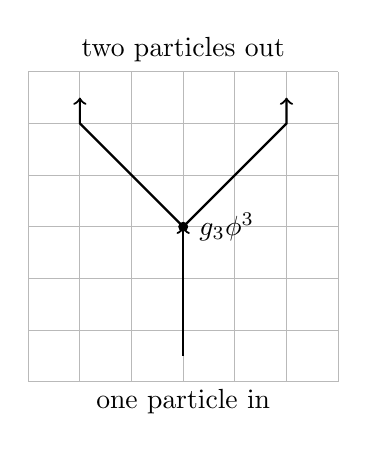
\begin{tikzpicture}[scale=0.82]
\draw[step=0.8,gray!55,thin] (0,0) grid (4.8,4.8);
\draw[thick,->] (2.4,0.4) -- (2.4,1.2) -- (2.4,2.0) -- (2.4,2.4);
\fill (2.4,2.4) circle (2.2pt);
\draw[thick,->] (2.4,2.4) -- (1.6,3.2) -- (0.8,4.0) -- (0.8,4.4);
\draw[thick,->] (2.4,2.4) -- (3.2,3.2) -- (4.0,4.0) -- (4.0,4.4);
\node[right] at (2.5,2.4) {$g_3\phi^3$};
\node at (2.4,-0.3) {one particle in};
\node at (2.4,5.15) {two particles out};
\end{tikzpicture}
\caption{Faktoren zweiter Ordnung transportieren ein Teilchen zu einem kubischen Aufspaltungsknoten und von ihm weg.}
\end{figure}

Auch eine Amplitude, bei der anfangs und am Ende jeweils ein Teilchen vorliegt, ist nicht mehr bloß eine Summe einzelner ununterbrochener Routen. Ein Beitrag ist die direkte Ausbreitung entlang einer Kette quadratischer Hüpfer. Ein anderer Beitrag enthält zwei kubische Faktoren: Das Teilchen spaltet sich in zwei auf, die sich später wieder vereinigen. Der Zwischenzustand kann daher mehr Teilchen enthalten als der äußere Zustand.\footnote{Die beiden Möglichkeiten werden anhand des Diagramms bei 01:09:44--01:11:36 rekonstruiert.}

\begin{figure}[htbp]
\centering
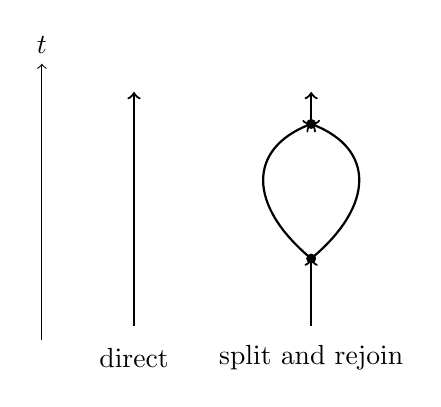
\begin{tikzpicture}[scale=0.9]
\draw[->] (-0.7,0) -- (-0.7,3.9) node[above] {$t$};
\draw[thick,->] (0.6,0.2) -- (0.6,3.5);
\node at (0.6,-0.25) {direct};
\draw[thick,->] (3.1,0.2) -- (3.1,1.15);
\fill (3.1,1.15) circle (2pt);
\draw[thick,->] (3.1,1.15) .. controls (2.2,1.9) and (2.2,2.7) .. (3.1,3.05);
\draw[thick,->] (3.1,1.15) .. controls (4.0,1.9) and (4.0,2.7) .. (3.1,3.05);
\fill (3.1,3.05) circle (2pt);
\draw[thick,->] (3.1,3.05) -- (3.1,3.5);
\node at (3.1,-0.25) {split and rejoin};
\end{tikzpicture}
\caption{Direkte Ausbreitung und ein Beitrag mit Aufspaltung--und Wiedervereinigung zur selben Einteilchenamplitude.}
\end{figure}

In der Elektrodynamik entspricht dem das Beispiel eines Elektrons, das ein Photon emittiert und später wieder absorbiert. Diese Emissions- und Absorptionsgeschichte ist Teil der Amplitude dafür, dass sich das Elektron von einem Punkt zu einem anderen ausbreitet. Höhere Ordnungen enthalten mehrere Emissionen und Absorptionen. Ein Photon kann sich in ein Elektron--Positron-Paar umwandeln, und das Elektron und das Positron dieses Zwischenpaares können ihrerseits ein Photon austauschen. Die Teilchen im Zwischenzustand müssen nicht einfach zusammengesetzt sein, nur weil der Teilcheninhalt am Anfang und am Ende einfach ist.\footnote{Die folgenden Beispiele der Rekonstruktion finden sich bei 01:11:22--01:12:34.}

\begin{figure}[htbp]
\centering
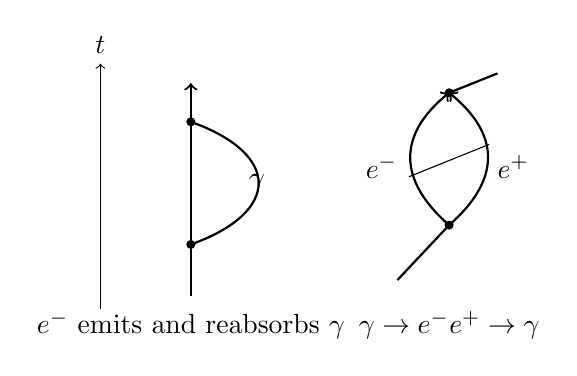
\begin{tikzpicture}[scale=0.82]
\draw[->] (-0.6,0) -- (-0.6,3.8) node[above] {$t$};
\draw[thick,->] (0.8,0.2) -- (0.8,3.5);
\fill (0.8,1.0) circle (2pt);
\fill (0.8,2.9) circle (2pt);
\draw[thick] (0.8,1.0) .. controls (2.2,1.5) and (2.2,2.4) .. (0.8,2.9);
\node[right] at (1.55,1.95) {$\gamma$};
\node at (0.8,-0.25) {$e^-$ emits and reabsorbs $\gamma$};
\draw[thick] (4.0,0.45) -- (4.8,1.3);
\fill (4.8,1.3) circle (2pt);
\draw[thick,->] (4.8,1.3) .. controls (4.0,2.0) and (4.0,2.7) .. (4.8,3.35);
\draw[thick,->] (4.8,1.3) .. controls (5.6,2.0) and (5.6,2.7) .. (4.8,3.35);
\fill (4.8,3.35) circle (2pt);
\draw[thick] (4.8,3.35) -- (5.55,3.65);
\draw[thin] (4.18,2.05) -- (5.42,2.55);
\node[left] at (4.15,2.2) {$e^-$};
\node[right] at (5.4,2.2) {$e^+$};
\node at (4.8,-0.25) {$\gamma\to e^-e^+\to\gamma$};
\end{tikzpicture}
\caption{Ein Beitrag zur Selbstemission eines Elektrons und eine Photonengeschichte mit einem Elektron--Positron-Paar.}
\end{figure}

Jede solche Geschichte ergibt sich aus einem bestimmten Produkt von Termen in der Entwicklung der Exponentialfunktion. Ihr Koeffizient enthält die passende Potenz von \(i\), eine Fakultät aus der Exponentialreihe und die an ihre Knoten gebundenen Kopplungen. Der Koeffizient liefert den Beitrag dieser Geschichte; die Amplitude für die angegebenen Anfangs- und Endzustände ist jedoch die Summe aller Geschichten mit denselben äußeren Zuständen.

\begin{classroomqa}
\lecturetimestamp{01:13:18}
\audiencequestion{Kann derselbe Gesamtprozess in mehreren verschiedenen Geschichten ablaufen, sodass sie alle zu seiner Amplitude beitragen?}
\lecturerresponse{Ja. Die Amplitude des Prozesses ergibt sich aus allen verschiedenen Geschichten, die denselben Anfangszustand mit demselben Endzustand verbinden.}
\end{classroomqa}

Es gibt also zwei gleichwertige Arten, Quantenfeldtheorie zu organisieren. In der Feldbeschreibung gibt man eine Anfangs- und eine Endfeldkonfiguration vor und summiert über alle dazwischenliegenden Feldgeschichten. In der Teilchenbeschreibung wird das Feld in Quanten aufgelöst: Man gibt den einlaufenden und auslaufenden Teilcheninhalt vor und summiert über alle Teilchengeschichten, die beide verbinden. Beiden Beschreibungen liegt dieselbe Lagrangefunktion zugrunde.

\section{Quartische Terme, Erhaltungssätze und Kopplungen}

Eine quartische Wechselwirkung,
\begin{equation}
\mathcal{L}_{\mathrm{int}}=g_4\phi^4,
\end{equation}
hat an einem Punkt vier Feldfaktoren. Zu ihren lokalen Teilchenlesarten gehören
\begin{equation}
\begin{gathered}
2\longrightarrow2,
\qquad
1\longrightarrow3,
\qquad
3\longrightarrow1,\\
0\longrightarrow4,
\qquad
4\longrightarrow0.
\end{gathered}
\end{equation}
Ein einzelner Knoten mit vier Beinen kann also Zweiteilchenstreuung, die Aufspaltung eines Teilchens in drei, die Vereinigung von drei Teilchen zu einem oder die Orientierung aller vier Beine nach außen oder nach innen beschreiben.\footnote{Die Orientierungen werden anhand des Diagramms bei 01:14:28--01:15:18 rekonstruiert.}

\begin{figure}[htbp]
\centering
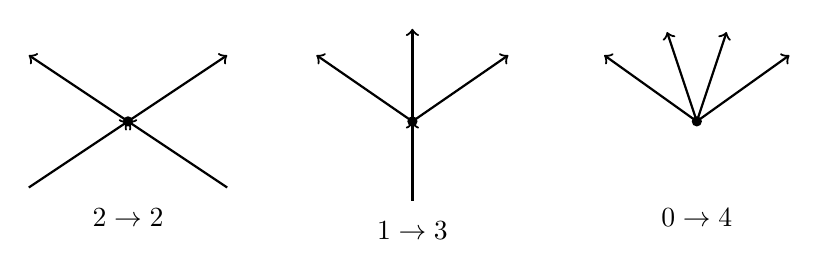
\begin{tikzpicture}[scale=0.84]
\fill (0,0) circle (2.2pt);
\draw[thick,->] (-1.5,-1.0) -- (0,0);
\draw[thick,->] (1.5,-1.0) -- (0,0);
\draw[thick,->] (0,0) -- (-1.5,1.0);
\draw[thick,->] (0,0) -- (1.5,1.0);
\node at (0,-1.45) {$2\to2$};
\begin{scope}[xshift=4.3cm]
\fill (0,0) circle (2.2pt);
\draw[thick,->] (0,-1.2) -- (0,0);
\draw[thick,->] (0,0) -- (-1.45,1.0);
\draw[thick,->] (0,0) -- (0,1.4);
\draw[thick,->] (0,0) -- (1.45,1.0);
\node at (0,-1.65) {$1\to3$};
\end{scope}
\begin{scope}[xshift=8.6cm]
\fill (0,0) circle (2.2pt);
\draw[thick,->] (0,0) -- (-1.4,1.0);
\draw[thick,->] (0,0) -- (-0.45,1.35);
\draw[thick,->] (0,0) -- (0.45,1.35);
\draw[thick,->] (0,0) -- (1.4,1.0);
\node at (0,-1.45) {$0\to4$};
\end{scope}
\end{tikzpicture}
\caption{Drei lokale Orientierungen eines Wechselwirkungsknotens mit vier Beinen.}
\end{figure}

Die lokale Lesart \(0\to4\) besagt für sich genommen nicht, dass vier Teilchen als physikalischer Prozess spontan aus dem Vakuum entstehen können. Der Knoten muss weiterhin über alle möglichen Raumzeitpunkte summiert werden. Kann der vorgeschlagene äußere Zustand die Energie nicht erhalten, heben sich die Phasenbeiträge dieser Punkte auf.

\begin{classroomqa}
\lecturetimestamp{01:15:18}
\audiencequestion{Beschreibt die Orientierung mit vier ausgehenden Linien, dass spontan vier Teilchen im Endzustand entstehen?}
\lecturerresponse{Das ist eine lokale Lesart des Operators mit vier Feldern; ein Prozess ohne einlaufende Energie verletzt jedoch die Energieerhaltung. Addiert man die Amplituden für alle möglichen Raumzeitpunkte des Knotens, heben sie sich zu null auf.}
\end{classroomqa}

\begin{classroomqa}
\lecturetimestamp{01:15:58}
\audiencequestion{Ergeben sich die Energie- und Impulserhaltung aus der Rechnung selbst?}
\lecturerresponse{Ja. Die Integration des Knotens über die gesamte Zeit erzwingt die Energieerhaltung, die Integration über den gesamten Raum die Impulserhaltung. Die Summe über die Positionen des Knotens verschwindet, sofern nicht beides erhalten ist.}
\end{classroomqa}

Unter Berücksichtigung dieser Erhaltungssätze trägt jedes nach der Lagrangefunktion erlaubte Diagramm eine gewisse Amplitude bei. Die Größe dieses Beitrags hängt zum Teil vom Koeffizienten des jeweiligen Wechselwirkungsterms ab. Bezeichnen wir die kubischen und quartischen Koeffizienten mit \(G_3\) bzw. \(G_4\). Jeder Knoten mit drei Beinen liefert einen Faktor \(G_3\), jeder Knoten mit vier Beinen einen Faktor \(G_4\). Die schematische Kopplungsabhängigkeit eines Diagramms mit \(V_3\) kubischen und \(V_4\) quartischen Knoten lautet daher
\begin{equation}
\mathcal{A}_{\mathrm{graph}}
\propto G_3^{V_3}G_4^{V_4}.
\end{equation}

Sind diese Kopplungen klein, trägt ein Diagramm mit wenigen Knoten im Allgemeinen mehr bei als eines mit vielen Knoten. Jeder zusätzliche Knoten bringt einen weiteren kleinen Faktor mit sich. Dadurch kann die störungstheoretische Summe nützlich sein: Man beginnt mit den einfachsten Diagrammen und fügt dann nacheinander immer kleinere Korrekturen hinzu.

Ob die vollständige Reihe tatsächlich konvergiert, ist eine schwierige Frage. Kleine Kopplungen machen die Ordnung der Beiträge plausibel, lösen aber nicht von selbst alle Konvergenzprobleme. Bei großen Kopplungen kann die naive Reihe vollständig versagen. Das zeigt nicht, dass die zugrunde liegende Theorie falsch ist; möglicherweise ist lediglich die Entwicklung nach Potenzen der Kopplung eine ungeeignete Berechnungsmethode. Die hier besprochenen Verfahren sind unmittelbar am nützlichsten, wenn die Kopplungen so klein sind, dass ein Diagramm mit vier Knoten viel kleiner ist als eines mit zwei.

\begin{classroomqa}
\lecturetimestamp{01:19:24}
\audiencequestion{Lässt sich die Farbtheorie auf dieselbe Weise behandeln?}
\lecturerresponse{Ja. Die Farbtheorie lässt sich auf dieselbe Weise formulieren und wird später besprochen.}
\end{classroomqa}

\section{Propagatoren, Knoten und komplementäre Beschreibungen}

Als Nächstes müssen die Teilchen aufgelistet und ihre Dynamik entweder durch eine Lagrangefunktion oder durch Feynmanregeln kodiert werden. Das sind zwei Formen derselben Information. Quadratische Terme beschreiben die Ausbreitung von einem Punkt zu einem anderen. Eine Linie, die diese Ausbreitung darstellt, heißt Propagator. Terme mit drei oder mehr Feldern beschreiben Stellen, an denen Linien zusammentreffen. Diese Treffpunkte heißen Knoten. Zum Beispiel:
\begin{equation}
\begin{aligned}
\text{quadratic term}
&\longleftrightarrow \text{propagator},\\
G_3\phi^3
&\longleftrightarrow \text{three-leg vertex}.
\end{aligned}
\end{equation}

Man kann eine Theorie festlegen, indem man für jedes Teilchen ein Quantenfeld angibt und eine Lagrangefunktion mit allen Massen und Wechselwirkungen aufschreibt. Gleichwertig dazu kann man alle Propagatoren, alle erlaubten Knoten und die zu jedem Knoten gehörenden Koeffizienten auflisten. Beide Listen geben an, welche Prozesse möglich sind und wie sich den zugehörigen Diagrammen Amplituden zuordnen lassen.

Zum Beispiel können zwei Elektronen durch den Austausch eines Photons streuen. Jede Elektronenlinie enthält einen Elektron--Elektron--Photon-Knoten, und der Photonpropagator verbindet die beiden Knoten.\footnote{Das Diagramm wird anhand des Beispiels bei 01:21:38 rekonstruiert.}

\begin{figure}[htbp]
\centering
\begin{tikzpicture}[scale=0.95]
\draw[->] (-0.6,-0.2) -- (0.2,1.4);
\draw[->] (0.2,1.4) -- (-0.7,3.1);
\draw[->] (3.5,-0.2) -- (2.7,1.4);
\draw[->] (2.7,1.4) -- (3.6,3.1);
\fill (0.2,1.4) circle (2pt);
\fill (2.7,1.4) circle (2pt);
\draw[thick] (0.2,1.4) -- (2.7,1.4);
\node[above] at (1.45,1.4) {$\gamma$};
\node[left] at (-0.2,0.5) {$e^-$};
\node[right] at (3.1,0.5) {$e^-$};
\end{tikzpicture}
\caption{Zweielektronenstreuung durch den Austausch eines Photons.}
\end{figure}

Die Lagrangefunktion bestimmt die Amplitude dieses Diagramms und enthält die Symmetrien und Erhaltungssätze, die sie einschränken. In einer nach der Zeit orientierten Zeichnung bilden die unten eingezeichneten Teilchen die Anfangskonfiguration, die oben eingezeichneten die Endkonfiguration.

\begin{classroomqa}
\lecturetimestamp{01:22:06}
\audiencequestion{Sind in einem Feynman-Diagramm die Teilchen unten die Anfangskonfiguration und die oben die Endkonfiguration?}
\lecturerresponse{Ja. Unten ist die Anfangskonfiguration der Teilchen, oben die Endkonfiguration.}
\end{classroomqa}

Teilchen- und Feldbeschreibung sind komplementär, ähnlich wie Impuls- und Ortsbeschreibung in der gewöhnlichen Quantenmechanik. Sie beschreiben dasselbe System in verschiedenen Basen. Dazu gehört auch eine entsprechende Unschärfe: Ist die Teilchenzahl genau festgelegt, ist der Feldwert unbestimmt; ist der Feldwert genau festgelegt, ist die Teilchenzahl unbestimmt. Keine der beiden Beschreibungen ersetzt die andere, und die Lagrangefunktion ist für beide nützlich.

\begin{classroomqa}
\lecturetimestamp{01:23:26}
\audiencequestion{Werden die Kopplungskonstanten von der Theorie vorhergesagt oder experimentell bestimmt?}
\lecturerresponse{Symmetrien können manchmal eine Kopplungskonstante mit einer anderen in Beziehung setzen; ihre Zahlenwerte stammen im Allgemeinen jedoch aus dem Experiment.}
\end{classroomqa}

\section{Gemessene Eingangsgrößen und weitreichende Vorhersagen}

Die Quantenfeldtheorie selbst ist elegant und schön. Doch sobald man die Fakten auflistet---welche Teilchen es gibt, welche Massen sie haben und wie groß ihre Kopplungskonstanten sind---, ergibt sich ein Durcheinander. Es ist ein sehr hässliches Durcheinander, das abgesehen von der durch Symmetrien gestifteten Ordnung kaum Zusammenhang aufweist. Symmetrien setzen verschiedene Teilchenarten und ihre Prozesse miteinander in Beziehung, allerdings nur in begrenztem Umfang. Ein großer Teil des Inventars bleibt eine umfangreiche Sammlung vergleichsweise zufälliger Fakten über eine wenig motivierte Ansammlung verschiedener Teilchenarten.

\begin{classroomqa}
\lecturetimestamp{01:24:58}
\audiencequestion{Warum kann man den gemessenen Kopplungskonstanten so sehr vertrauen?}
\lecturerresponse{Ist eine Kopplung gemessen, führt eine Änderung ihres Werts zu falschen Vorhersagen. Ihr Wert wird durch die vielen Berechnungen geprüft, in die er eingeht.}
\end{classroomqa}

Es gibt zu viele Teilchen, also zu viele Felder---zu viele für jeden ästhetischen Maßstab. Es sind ungefähr hundert oder mehr. Es gibt viele Kopplungskonstanten, mehr oder weniger aus dem Experiment entnommene Zahlen, und zahlreiche Massen, die über den gesamten Wertebereich verteilt sind. Zwischen ihnen bestehen einige Beziehungen, aber nur wenige.

Sobald man diese Größen kennt, kann man mit den Berechnungen beginnen. Sobald man sie kennt, kann man alles über diese Teilchen mit großer Präzision berechnen. Alles über Quarks, Elektronen, Photonen und den Rest reicht bis in die Atomphysik, Teilchenphysik, Kernphysik, Chemie und vielleicht auch Biologie hinein. Die Zahl der Eingangsgrößen mag größer sein, als einem lieb ist, aber die Zahl der möglichen Ergebnisse ist enorm.

\section{Quantenelektrodynamik als Beispiel für Störungstheorie}

Die Quantenelektrodynamik liefert ein konkretes Beispiel für die Entwicklung nach der Kopplung.

\begin{classroomqa}
\lecturetimestamp{01:26:12}
\audiencequestion{Wie viele Wechselwirkungskopplungen vom Typ \(G_n\) gibt es für Elektronen und Photonen?}
\lecturerresponse{Es gibt eine elementare Wechselwirkungskopplung: die elektrische Ladung \(e\). Sie ist ein Koeffizient vom Typ \(G_3\), der einem Knoten zugeordnet ist, an dem ein Elektron eintritt, ein Elektron austritt und ein Photon emittiert oder absorbiert wird.}
\end{classroomqa}

Unterdrückt man die Spinormatrizen und Indizes, hat die Wechselwirkung schematisch folgenden Feldinhalt:
\begin{equation}
\mathcal{L}_{\mathrm{QED,int}}
\sim e\,(\text{electron bilinear})\,A,
\end{equation}
wobei \(A\) das Photonenfeld bezeichnet. Für das Abzählungsargument ist die genaue Dirac-Matrixstruktur nicht erforderlich. Die elementare QED-Regel beschreibt die Emission oder Absorption eines Photons durch ein Elektron; alle komplizierteren QED-Diagramme setzen sich aus wiederholten Anwendungen dieses einen Knotens zusammen.\footnote{Der schematische Knoten wird anhand von 01:26:42 rekonstruiert; in der Quelle ist die genaue Matrixstruktur bewusst unterdrückt.}

\begin{figure}[htbp]
\centering
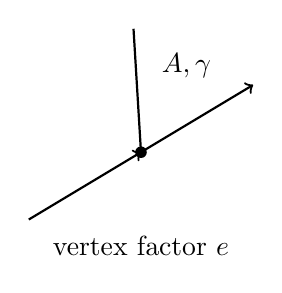
\begin{tikzpicture}[scale=0.95]
\draw[thick,->] (-1.5,-0.9) -- (0,0);
\draw[thick,->] (0,0) -- (1.5,0.9);
\draw[thick] (0,0) -- (-0.1,1.65);
\fill (0,0) circle (2.2pt);
\node[right] at (0.15,1.15) {$A,\gamma$};
\node at (0,-1.25) {vertex factor $e$};
\end{tikzpicture}
\caption{Der elementare Elektron--Elektron--Photon-Knoten der Quantenelektrodynamik.}
\end{figure}

\begin{classroomqa}
\lecturetimestamp{01:27:38}
\audiencequestion{Wie sieht es mit der Elektron--Proton-Streuung aus?}
\lecturerresponse{In der elementaren Behandlung des Atoms kann man das Proton als feststehende, unendlich schwere Punktquelle idealisieren---als schweres Teilchen, das an seinem Platz festgenagelt ist. Seine eigene quantenfeldtheoretische Dynamik wird erst berücksichtigt, wenn man die innere Theorie der Protonen und Neutronen einbezieht.}
\end{classroomqa}

\begin{classroomqa}
\lecturetimestamp{01:28:30}
\audiencequestion{Kann sich das Elektron relativ zu diesem Proton beinahe mit Lichtgeschwindigkeit bewegen?}
\lecturerresponse{Ja.}
\end{classroomqa}

Betrachten wir die Photonstreuung an einem Elektron. In niedrigster Ordnung enthält das Diagramm zwei Elektron--Elektron--Photon-Knoten. Die Amplitude ist daher proportional zu \(e^2\):
\begin{equation}
\mathcal{A}_{\mathrm{lowest}}\propto e^2.
\end{equation}
Die Wahrscheinlichkeit oder gleichwertig die Kopplungsabhängigkeit des Wirkungsquerschnitts ergibt sich aus dem Betragsquadrat und ist proportional zu \(e^4\):
\begin{equation}
P_{\mathrm{lowest}}\ \text{or}\ \sigma_{\mathrm{lowest}}
\propto e^4.
\end{equation}
Bei der üblichen dimensionslosen Normierung ist die elektrische Kopplung klein. Daher ist eine tatsächliche Streuung viel unwahrscheinlicher, als dass das Photon einfach ohne Streuung vorbeifliegt.

In dieser Ordnung gibt es bereits zwei Diagramme. Bei der einen zeitlichen Reihenfolge wird das einlaufende Photon absorbiert und später das auslaufende Photon emittiert. Bei der anderen wird das auslaufende Photon emittiert, bevor das einlaufende Photon absorbiert wird. Beide Amplituden tragen bei.\footnote{Die beiden zeitlichen Reihenfolgen werden anhand der Diagramme bei 01:28:42 und 01:30:18 rekonstruiert.}

\begin{figure}[htbp]
\centering
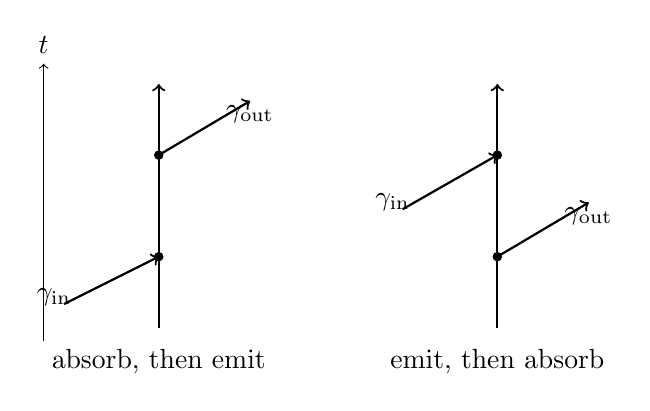
\begin{tikzpicture}[scale=0.86]
\draw[->] (-0.7,0) -- (-0.7,4.1) node[above] {$t$};
\draw[thick,->] (1.0,0.2) -- (1.0,3.8);
\fill (1.0,1.25) circle (2pt);
\fill (1.0,2.75) circle (2pt);
\draw[thick,->] (-0.4,0.55) -- (1.0,1.25);
\draw[thick,->] (1.0,2.75) -- (2.35,3.55);
\node[left] at (-0.15,0.65) {$\gamma_{\mathrm{in}}$};
\node[right] at (1.85,3.35) {$\gamma_{\mathrm{out}}$};
\node at (1.0,-0.3) {absorb, then emit};
\begin{scope}[xshift=5.0cm]
\draw[thick,->] (1.0,0.2) -- (1.0,3.8);
\fill (1.0,1.25) circle (2pt);
\fill (1.0,2.75) circle (2pt);
\draw[thick,->] (1.0,1.25) -- (2.35,2.05);
\draw[thick,->] (-0.4,1.95) -- (1.0,2.75);
\node[right] at (1.85,1.85) {$\gamma_{\mathrm{out}}$};
\node[left] at (-0.15,2.05) {$\gamma_{\mathrm{in}}$};
\node at (1.0,-0.3) {emit, then absorb};
\end{scope}
\end{tikzpicture}
\caption{Die beiden zeitlichen Reihenfolgen niedrigster Ordnung für die Elektron--Photon-Streuung.}
\end{figure}

Die Amplitude niedrigster Ordnung ist folglich nicht ein einzelnes Diagramm, sondern die Summe der beiden:
\begin{equation}
\begin{aligned}
\mathcal{A}^{(2)}
&=
\mathcal{A}_{\mathrm{absorb\ then\ emit}}
+\mathcal{A}_{\mathrm{emit\ then\ absorb}},\\
\mathcal{A}^{(2)}&\propto e^2.
\end{aligned}
\end{equation}

Korrekturen höherer Ordnung fügen weitere elementare Knoten hinzu. Ein zusätzliches internes Photon, das an zwei Stellen an die Elektronenlinie gekoppelt ist, bringt zwei Faktoren \(e\) hinzu. Der Beitrag ist damit in der Amplitude proportional zu \(e^4\) und in ihrem Betragsquadrat proportional zu \(e^8\). Eine Photonlinie kann auch eine Elektron--Positron-Einfügung enthalten, die wiederum elementare Knoten und zusätzliche Potenzen von \(e\) hinzufügt. Das sind Beispiele, keine vollständige Aufzählung; das zusätzliche Photon kann an vielen Stellen angefügt werden.\footnote{Die Strukturen höherer Ordnung werden anhand von 01:30:38--01:31:16 rekonstruiert.}

\begin{figure}[htbp]
\centering
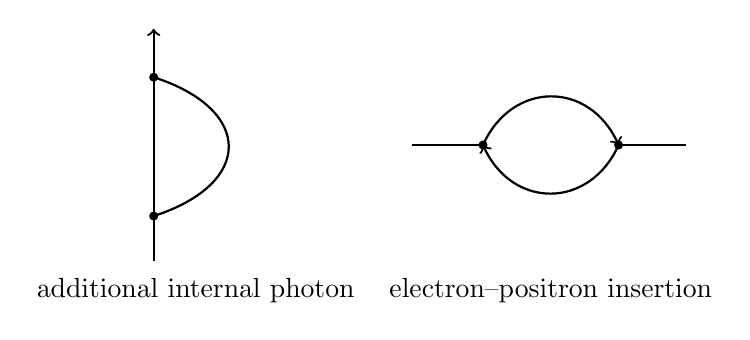
\begin{tikzpicture}[scale=0.82]
\draw[thick,->] (0.9,0.2) -- (0.9,3.8);
\fill (0.9,0.9) circle (2pt);
\fill (0.9,3.05) circle (2pt);
\draw[thick] (0.9,0.9) .. controls (2.45,1.4) and (2.45,2.55) .. (0.9,3.05);
\node at (1.55,-0.25) {additional internal photon};
\begin{scope}[xshift=5.1cm]
\draw[thick] (-0.2,2.0) -- (0.9,2.0);
\fill (0.9,2.0) circle (2pt);
\fill (3.0,2.0) circle (2pt);
\draw[thick,->] (0.9,2.0) .. controls (1.35,3.0) and (2.55,3.0) .. (3.0,2.0);
\draw[thick,->] (3.0,2.0) .. controls (2.55,1.0) and (1.35,1.0) .. (0.9,2.0);
\draw[thick] (3.0,2.0) -- (4.05,2.0);
\node at (1.95,-0.25) {electron--positron insertion};
\end{scope}
\end{tikzpicture}
\caption{Zwei QED-Strukturen höherer Ordnung, die elementare Knoten und weitere Potenzen von \(e\) hinzufügen.}
\end{figure}

Die QED-Entwicklung schreitet somit in aufeinanderfolgenden Potenzen von \(e^2\) voran. Jede vergleichbar neue Komplikation fügt der Amplitude zwei Potenzen der elektrischen Ladung hinzu. Bei der verwendeten Normierung ist eine solche Korrektur in der Amplitude ungefähr hundert- oder zweihundertmal kleiner als die vorherige Ordnung. Die komplizierteren Diagramme werden zunehmend schwächer, sodass die störungstheoretische Summe nützlich sein kann.

Die Wahrscheinlichkeit erhält man nicht, indem man jedes Diagramm einzeln quadriert und anschließend diese Quadrate addiert. Zuerst addiert man alle Amplituden, die zum selben äußeren Prozess beitragen:
\begin{equation}
\mathcal{A}_{\mathrm{total}}=\sum_r\mathcal{A}_r.
\end{equation}
Erst dann bildet man
\begin{equation}
P=\left|\mathcal{A}_{\mathrm{total}}\right|^2
=\left|\sum_r\mathcal{A}_r\right|^2.
\end{equation}
Die Kreuzterme zwischen verschiedenen Diagrammen sind Interferenzterme. Die Regel ist einfach und wesentlich: zuerst addieren, dann quadrieren.

\section{Auf dem Weg zum Teilcheninventar und zum Standardmodell}

Mit Propagatoren, Knoten, dem Abzählen der Kopplungen und der Interferenz kann die Beschreibung der Teilchenphysik nun richtig beginnen. Man kann die Teilchen benennen, ihre Massen angeben, die Lagrangefunktionen aufschreiben, die sie teils theoretisch und teils experimentell festlegen, und ihre Symmetrien unmittelbar in diesen Lagrangefunktionen untersuchen. Derselbe Rahmen führt dann zum Standardmodell und seinen Eigenschaften.

\begin{classroomqa}
\lecturetimestamp{01:33:22}
\audiencequestion{Kann der konstante Massenkoeffizient \(m^2\) durch das Higgs-Feld ersetzt werden?}
\lecturerresponse{Ja. Das ist der richtige Gedanke; der Mechanismus wird später besprochen.}
\end{classroomqa}

\begin{classroomqa}
\lecturetimestamp{01:33:42}
\audiencequestion{Können die benachbarten Gitterpunkte \(x\) und \(x'\) zu zwei verschiedenen Zeiten liegen?}
\lecturerresponse{Ja. Sie können in Zeitrichtung benachbart sein; so wird die vertikale Ausbreitung auf dem Gitter dargestellt.}
\end{classroomqa}

Das Quadrat der Differenz für benachbarte Punkte enthält sowohl Terme am selben Ort als auch Kreuzterme über einen Link:
\begin{equation}
\bigl[\phi(x)-\phi(x')\bigr]^2
=
\phi(x)^2+\phi(x')^2-2\phi(x)\phi(x').
\end{equation}

\begin{classroomqa}
\lecturetimestamp{01:33:56}
\audiencequestion{Welcher Term beschreibt ein Teilchen, das einfach stillsteht?}
\lecturerresponse{Die Terme am selben Ort \(\phi(x)^2\) und \(\phi(x')^2\) im Quadrat der Differenz beschreiben den Stillstand, während der Kreuzterm \(\phi(x)\phi(x')\) die Interpretation als Bewegung liefert. Auch der explizite Massenterm trägt Faktoren bei, die einem Stillstand am selben Ort entsprechen.}
\end{classroomqa}
